\documentclass{standalone}
\usepackage{fontspec}
\setmainfont{CardCharacters}

\usepackage[dvipsnames]{xcolor}
\usepackage{tikz}

\newcommand{\myten}{\textcolor{black}{=}}
\newcommand{\myclub}{\textcolor{black}{]}}
\newcommand{\mydiamond}{\textcolor{red}{[}}
\newcommand{\myheart}{\textcolor{red}{\{}}
\newcommand{\myspade}{\textcolor{black}{\}}}

\begin{document}
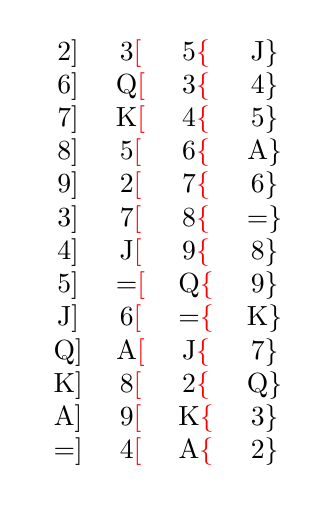
\begin{tikzpicture}
\node at (0,0) {
\begin{tabular}{cccc}
2\myclub & 3\mydiamond & 5\myheart & J\myspade \\
6\myclub & Q\mydiamond & 3\myheart & 4\myspade \\
7\myclub & K\mydiamond & 4\myheart & 5\myspade \\
8\myclub & 5\mydiamond & 6\myheart & A\myspade \\
9\myclub & 2\mydiamond & 7\myheart & 6\myspade \\
3\myclub & 7\mydiamond & 8\myheart & \myten\myspade \\
4\myclub & J\mydiamond & 9\myheart & 8\myspade \\
5\myclub & \myten\mydiamond & Q\myheart & 9\myspade \\
J\myclub & 6\mydiamond & \myten\myheart & K\myspade \\
Q\myclub & A\mydiamond & J\myheart & 7\myspade \\
K\myclub & 8\mydiamond & 2\myheart & Q\myspade \\
A\myclub & 9\mydiamond & K\myheart & 3\myspade \\
\myten\myclub & 4\mydiamond & A\myheart & 2\myspade \\
\end{tabular}
};
\end{tikzpicture}
\end{document}